\documentclass[11pt, a4paper,listof=totoc, bibliography=totoc, numbers=noenddot]{scrreprt}
\usepackage[T1]{fontenc}
\usepackage[utf8]{inputenc}
\usepackage[a4paper, top=25mm, left=25mm, right=20mm, bottom=25mm, footskip=12mm]{geometry}
\usepackage{amsmath}
\usepackage{mathtools}
\DeclarePairedDelimiter\abs{\lvert}{\rvert}%Absolut Brackets with resizing
\DeclarePairedDelimiter\norm{\lVert}{\rVert}%Norm Brackets with resizing

\usepackage[]{acronym}
\usepackage{csquotes}
%\usepackage{cite}


\usepackage[backend=biber, sorting=anyt, maxnames=99, maxcitenames=3,sortcites=true, hyperref=true, bibstyle=alphabetic, citestyle=alphabetic]{biblatex}
\DeclareNameAlias{author}{last-first} 
\renewcommand*{\multinamedelim}{\addsemicolon\space}   
\renewcommand*{\finalnamedelim}{\addsemicolon\space} 
\renewcommand*{\labelnamepunct}{\addcolon\addspace}
%\DeclareFieldFormat{url}{\mkbibbrackets{Online}\addspace\url{#1}}
\DeclareFieldFormat{url}{URL: \addspace\url{#1}}
\DeclareFieldFormat{urldate}{\mkbibbrackets{#1}}
\DeclareFieldFormat{edition}{Auflage~{#1}}
\DeclareFieldFormat{volume}{Band~{#1}}
\addbibresource{Struktur/Literaturverzeichnis.bib}




\usepackage[ngerman]{babel}
\usepackage{lmodern}
\renewcommand*\familydefault{\sfdefault}
\usepackage[cm]{sfmath}     %serifenlose Matheumgebung
%\usepackage[eulergreek]{sansmath}  %andere serifenlose Matheschriftart
%\sansmath
\usepackage{amssymb}
\usepackage{amsmath}
\allowdisplaybreaks % \displaybreak an Stelle von Seitenumbruch
%\DeclareMathOperator{\lg}{lg}


\usepackage{relsize}
\usepackage{amsfonts}
\usepackage{textcomp}
\usepackage{url}


\newcommand\tab[1][1,5cm]{\hspace*{#1}}
\newcommand\halftab[1][0,5cm]{\hspace*{#1}}
\newcommand\halfsite[1][0.5\textwidth]{\hspace*{#1}}
\usepackage{graphicx}
\usepackage[onehalfspacing]{setspace}
\usepackage{wrapfig}
\usepackage{float}
\usepackage{array}
\usepackage{tabularx}
\usepackage{threeparttable}
\usepackage{multirow}
\usepackage{multicol}
\newcolumntype{C}[1]{>{\centering\arraybackslash}m{#1}}
\newcolumntype{R}[1]{>{\raggedleft\arraybackslash}p{#1}}
\usepackage{booktabs}
\usepackage{longtable} 


\usepackage{paralist}

\usepackage{subcaption}


\usepackage{pdfpages}


\usepackage{siunitx}
\sisetup{detect-weight, detect-family, output-decimal-marker = {,}, per-mode=symbol, bracket-unit-denominator=false, scientific-notation=false, locale = DE}
\DeclareSIUnit{\mpa}{MPa}
\DeclareSIUnit{\Decade}{Dekade}
\DeclareSIUnit{\HV}{HV}
\DeclareSIUnit{\Dezibel}{dB}

\usepackage{icomma}     % Komma als Trennzeichen statt Punkt (kein Abstand zwischen Ziffern und Komma in Zahl)



\newcommand{\acrounit}[1]{\acroextra{\makebox[25mm][l]{\si{#1}}}}       % Abstand zwischen Symbol, Einheit und Erklärung im Symbolverzeichnis

\usepackage{nicefrac}



\usepackage{fancyhdr}
\pagestyle{fancy}              % Pagestyle für normale Seiten
\fancyhf{}
\lhead{\leftmark}
\rhead{\thepage}
\renewcommand\chaptermark[1]{\markboth{\thechapter~\MakeUppercase{#1}}{}}
\renewcommand{\headrulewidth}{0.4pt}
\lfoot{}
\cfoot{Vermessung der Schirmdämpfung von Folien und Schäumen im Fernfeld}
\rfoot{}
\renewcommand{\footrulewidth}{0.4pt}
%\renewcommand*\chapterpagestyle{fancy}

\fancypagestyle{plain}{         % Pagestyle für Chapterseiten
    \fancyhf{}
    \rhead{\thepage}
    \renewcommand{\headrulewidth}{0.4pt}
    \lfoot{}
    \cfoot{Vermessung der Schirmdämpfung von Folien und Schäumen im Fernfeld}
    \rfoot{}
    \renewcommand{\footrulewidth}{0.4pt}}


\usepackage{hyphenat}   %Worttrennung festlegen




\usepackage{hyperref}   %Links im Dokument zu Kapiteln, etc. 
\hypersetup{
    colorlinks=false,
    linkcolor=blue,
    filecolor=magenta,      
    urlcolor=cyan,
    pdftitle={<Arbeitsname>},
    pdfauthor=Christoph Peter,
    bookmarksnumbered=true,
    hidelinks
}
\urlstyle{same}

\usepackage{cleveref}   %sollte letztes eingebundenes Packet sein, weil sonst nicht funktioniert (auf jeden Fall unter hyperref)




%----------------------------------------------------------------------------
%Komandos für Haupt- und Anhangsverzeichnis

\makeatletter% --> De-TeX-FAQ
\newcommand*{\maintoc}{% Hauptinhaltsverzeichnis
  \begingroup
    \@fileswfalse% kein neues Verzeichnis öffnen
    \renewcommand*{\appendixattoc}{% Trennanweisung im Inhaltsverzeichnis
      \value{tocdepth}=-10000 % lokal tocdepth auf sehr kleinen Wert setzen
    }%
    \tableofcontents% Verzeichnis ausgeben
  \endgroup
}
\newcommand*{\appendixtoc}{% Anhangsinhaltsverzeichnis
  \begingroup
    \edef\@alltocdepth{\the\value{tocdepth}}% tocdepth merken
    \setcounter{tocdepth}{-10000}% Keine Verzeichniseinträge
    \renewcommand*{\contentsname}{% Verzeichnisname ändern
      Anhang}%
    \renewcommand*{\appendixattoc}{% Trennanweisung im Inhaltsverzeichnis
      \setcounter{tocdepth}{\@alltocdepth}% tocdepth wiederherstellen
    }%
    \protect\KOMAoptions{chapterentrydots}  %Zeilen mit dots auffüllen
    \tableofcontents% Verzeichnis ausgeben
    \setcounter{tocdepth}{\@alltocdepth}% tocdepth wiederherstellen
  \endgroup
}
\newcommand*{\appendixattoc}{% Trennanweisung im Inhaltsverzeichnis
}
\g@addto@macro\appendix{% \appendix erweitern
  %\if@openright\cleardoublepage\else\clearpage\fi % Neue Seite
  \phantomsection  %Befehl für hyperref zum Erstellen eines Ankerpunktes im Anhangsverzeichnis
  \clearpage 
  \addcontentsline{toc}{chapter}{\appendixname}% Eintrag ins Hauptverzeichnis
  \addtocontents{toc}{\protect\appendixattoc}% Trennanweisung in die toc-Datei
}

\g@addto@macro\appendix{%
  %\pagenumbering{Roman}%
  \addtocontents{toc}{\protect\renewcommand*{\protect\@pnumwidth}{1.6em}}%Seitenzahlen im Anhangverzeichnis nicht über Seitenrand hinaus. Problem entstand durch die langen römischen Zahlen. Siehe auch: http://www.komascript.de/node/608
  % 1 em = Breite eines großem M in der aktuellen Schriftart
  % Wert für römische Seitenzahlen am besten auf etwa 3.5em setzen; Standardwert für arabische Seitenzahlen im Inhaltverzeichnis: ca. 1.6em
}
\makeatother

%----------------------------------------------------------------------------
%Zeilenskip nach Absätzen
\newcommand{\linespace}{6pt}


%----------------------------------------------------------------------------
%Commands für unterschiedliche Schreibweisen von Referenzen

\newcommand{\Abb}{Abbildung~}

\newcommand{\Abschnitt}{Abschnitt~}
\newcommand{\Abschnitte}{Abschnitte~}
\newcommand{\Abschnitten}{Abschnitten~}

\newcommand{\Anhang}{Anhang~}

\newcommand{\Tabelle}{Tabelle~}

\newcommand{\Gleichung}{Gleichung~}
\newcommand{\Gleichungen}{Gleichungen~}



%----------------------------------------------------------------------------
%Commands für römische Zahlen

\newcommand{\uproman}[1]{\uppercase\expandafter{\romannumeral#1}}
\newcommand{\lowroman}[1]{\romannumeral#1\relax}
%----------------------------------------------------------------------------
%Counter
%\newcounter{<Counter>}
%\renewcommand*\the<Counter>{\arabic{<Counter>}}
%\setcounter{<Counter>}{1}



%----------------------------------------------------------------------------





\begin{document}
\sffamily

%----------------------------------------------------------------------------
%Worttrennungen
\hyphenation{
elek-tro-ma-gne-tisch 
Wellen-feld
Fall-unter-schei-dung
Quelle
}


%Penalty für Worttrennungen
\hyphenpenalty=400


\pagenumbering{Roman}

\setlength{\parindent}{0pt}
\renewcommand{\arraystretch}{1.2}   %Abstand der Tabellenzeilen 

\setlength{\jot}{10pt}              %Abstand zwischen Gleichungen in align-Umgebung

\begin{titlepage}

\noindent \begin{center}
{\scshape\LARGE Technische Universität Dresden \par}
Fakultät Maschinenwesen \par
Institut für Luft- und Raumfahrttechnik
\par\end{center}

\noindent \vspace{1cm}


\noindent \begin{center}
\textbf{\huge Grosser Beleg} \vspace{2cm}
\par\end{center}{\Large \par}

\begin{tabular}{p{2.5cm} l}
\renewcommand{\arraystretch}{1}
    \Large Thema: & \Large \textbf{Entwurf und Qualifikation einer Box zur Vermessung der} \\
     & \Large \textbf{Schirmdämpfung von Folien und Schäumen im Fernfeld}
\end{tabular}

\vspace{1cm}

\begin{tabular}{p{6cm} l}
\renewcommand{\arraystretch}{1}
Bearbeiter: & Christoph Peter\\
Studiengang: & Luft- und Raumfahrttechnik \\
Matrikel-Nr.: & 4500982 \\
 & \\
Betreuender Hochschullehrer: & Prof. Dr. Martin Tajmar\\
 & Technische Universität Dresden \\
 & Fakultät Maschinenwesen \\
 & Institut für Luft- und Raumfahrttechnik\\
 & \\
 Betreuer: & Dipl.-Ing. Tilman Schüler \\
 & Technische Universität Dresden \\
 & Institut für Luft- und Raumfahrttechnik  \\
 &          \\
 & Dipl.-Ing. Marcel Weikert \\
 & Technische Universität Dresden \\
 & Institut für Luft- und Raumfahrttechnik \\
 & \\
Ort der Durchführung: & Technische Universität Dresden \\
 & Institut für Luft- und Raumfahrttechnik \\
 & Marschnerstraße 32, 01307 Dresden \\
 & \\
 Zeitraum: & 01.09.2019 - 29.02.2020

\end{tabular}

\end{titlepage}


\onehalfspacing

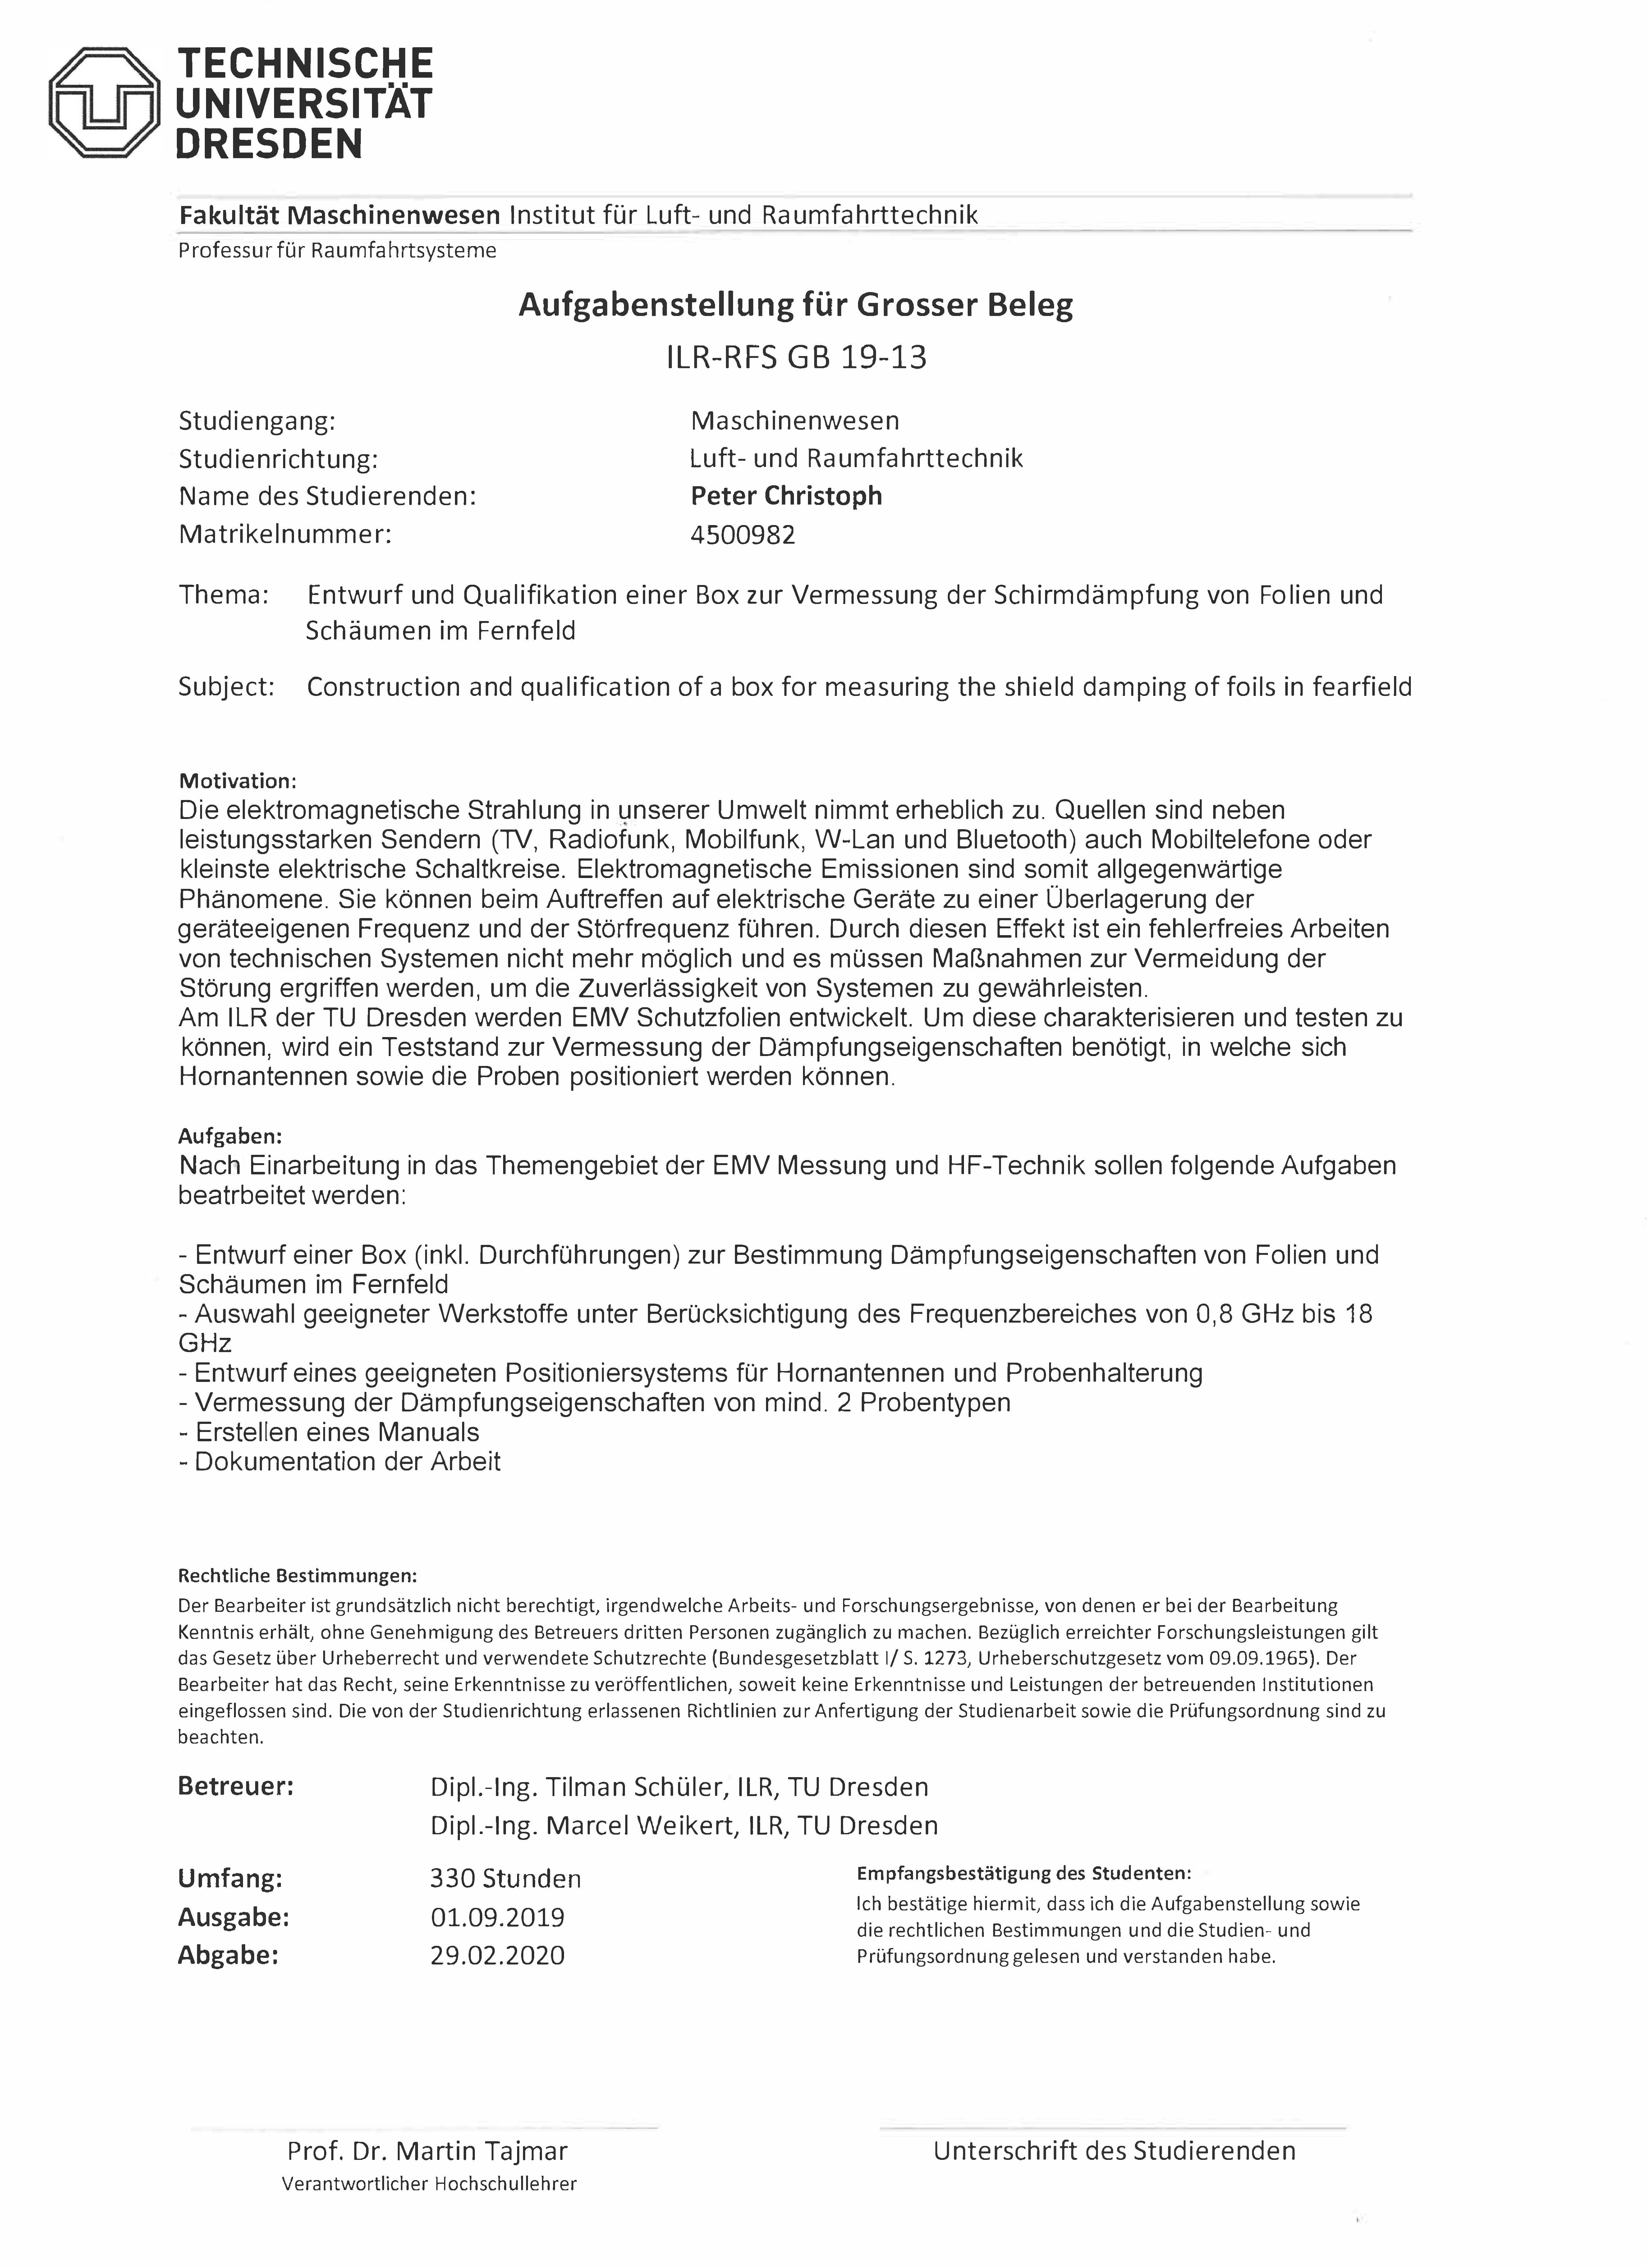
\includepdf[pages=-, offset= 0cm 0cm, pagecommand={\thispagestyle{empty}}, draft=true]{Struktur/Aufgabenstellung.pdf}

\chapter*{Selbstständigkeitserklärung}
\thispagestyle{empty}
%\addcontentsline{toc}{chapter}{Selbstständigkeitserklärung}

\vspace*{2cm}

\begin{large}
Hiermit erkläre ich, Christoph Peter, dass ich die vorliegende Arbeit mit dem Titel: \par
\vspace{1cm}
\begin{center}
    \Large \textbf{Entwurf und Qualifikation einer Box zur Vermessung der Schirmdämpfung von Folien und
Schäumen im Fernfeld} \par
\end{center} 
\vspace{1cm}
\noindent selbstständig verfasst habe. Es wurden keine anderen als die in der Arbeit angegebenen Quellen und Hilfsmittel benutzt. Die wörtlichen oder sinngemäß übernommenen Zitate habe ich als solche kenntlich gemacht.

\vspace{3cm}

\begin{tabular}{p{6cm}}
    \dotfill \\
    Christoph Peter \\[3cm]
    Dresden, den \today
\end{tabular}

\end{large}


\newpage

%\tableofcontents
\maintoc                %Hauptverzeichnis anstelle von \tableofcontents


\chapter*{Abkürzungsverzeichnis}
\addcontentsline{toc}{chapter}{Abkürzungsverzeichnis}
%\thispagestyle{fancy}
\markboth{Abkürzungsverzeichnis}{Abkürzungsverzeichnis} 

\noindent\rule{\textwidth}{0.5pt}
\textbf{Abkürzung} \hspace{18mm} \textbf{Erläuterung} \\[-\linespace]
\noindent\rule{\textwidth}{0.5pt}

\begin{acronym}[langesPlatzhalterwort]
%\acro{<Kurzform>}{<Langform>}
\acro{BW}{Bandbreite (Bandwidth)}
\acro{CE}{Europäische Konformität (Conformité Européenne)}
\acro{CNT}{Kohlenstoffnanoröhrchen (Carbon Nanotubes)}
\acro{DUT}{Prüfling (Device under Test)}
\acro{EMV}{Elektromagnetische Verträglichkeit}
    \acrodefplural{EMV}[EMV]{Elektromagnetischen Verträglichkeit}
\acro{F}{Forderung}
    \acrodefplural{F}[F]{Forderungen}
\acro{HF}{Hochfrequenz}
\acro{ILR}{Institut für Luft- und Raumfahrttechnik}
\acro{K}{Kriterium}
    \acrodefplural{K}[K]{Kriterien}
\acro{MSC}{Modenverwirbelungskammer (Mode Stirred Chamber)}
\acro{PU}{Polyurethan}
\acro{SMA}{Sub-Miniature-A}
\acro{TEM}{Transversalelektromagnetische Welle (Transverse Electromagnetic Mode)}
\acro{TUD}{Technische Universität Dresden}
\acro{VNA}{Vektorieller Netzwerkanalysator}
\acro{VSWR}{Stehwellenverhältnis (Voltage Standing Wave Ratio)}
\acro{W}{Wunsch}
    \acrodefplural{W}[W]{Wünsche}

\end{acronym}



\chapter*{Symbolverzeichnis}
\addcontentsline{toc}{chapter}{Symbolverzeichnis}
%\thispagestyle{fancy}
\markboth{Symbolverzeichnis}{Symbolverzeichnis}

\textit{Lateinische Symbole} \\[.5\linespace]
\noindent\rule{\textwidth}{0.5pt}
\textbf{Symbol} \hspace{12.5mm} \textbf{Einheit} \hspace{10.5mm} \textbf{Bezeichnung} \\[-\linespace]
\noindent\rule{\textwidth}{0.5pt}

\begin{acronym}[Platzhalterwort]

\acro{a}[$a(x,y,z,\ldots)$]{\acrounit{-}Allgemeines Skalarfeld}
\acro{A_P}[$A_P$]{\acrounit{\square\meter}Kondensatorplattenfläche}
\acro{vec_A}[$\vec A(x,y,z,\ldots)$]{\acrounit{-}Allgemeines Vektorfeld}


\acro{D}[$\vec D$]{\acrounit{\ampere\second\per\square\meter}Elektrische Flussdichte}

\acro{E}[$\vec E$]{\acrounit{\volt\per\meter}Elektrische Feldstärke}

\acro{F}[$\vec F_q$]{\acrounit{\newton}Kraft auf eine Ladung im elektrischen Feld}

\acro{n}[$\vec n_A$]{\acrounit{1}Normalenvektor auf der Fläche A}

\acro{q}[$q$]{\acrounit{\ampere\second}Elektrische Ladung}

\acro{x}[$x$]{\acrounit{-}Ortskoordinate im kartesischen Koordinatensystem}
\acro{y}[$y$]{\acrounit{-}Ortskoordinate im kartesischen Koordinatensystem}
\acro{z}[$z$]{\acrounit{-}Ortskoordinate im kartesischen Koordinatensystem}

\end{acronym}
\newpage



\textit{Griechische Symbole} \\[.5\linespace]
\noindent\rule{\textwidth}{0.5pt}
\textbf{Symbol} \hspace{12.5mm} \textbf{Einheit} \hspace{10.5mm} \textbf{Bezeichnung} \\[-\linespace]
\noindent\rule{\textwidth}{0.5pt}

\begin{acronym}[Platzhalterwort]

\acro{varepsilon}[$\varepsilon$]{\acrounit{\ampere\second\per\volt\per\meter}Dielektrizitätszahl}
\acro{varepsilon}[$\varepsilon_0$]{\acrounit{\ampere\second\per\volt\per\meter}Dielektrizitätszahl des leeren Raumes}
\acro{varepsilon}[$\varepsilon_r$]{\acrounit{1}Relative Dielektrizitätszahl}


\end{acronym}
\newpage


%\newcounter{savepage}
%\setcounter{savepage}{\arabic{page}}
\pagenumbering{arabic}





\chapter{Einleitung}\label{cha:1}

Der Begriff der \acp{EMV} ist nicht nur beim Entwurf und Aufbau von Satelliten und anderen Raumfahrzeugen, sondern auch im terestrischen Bereich ein Designtreiber, der immer mehr an Bedeutung gewinnt. Aufgrund des Vordringens elektronischer Komponenten und Baugruppen in immer mehr Bereiche alltäglicher Anwendungen erhöht sich in gleichem Maße nicht nur die Anzahl der potentiell störanfälligen Geräte, sondern auch die Zahl elektromagnetischer Störquellen. \par
\vspace{\linespace}
Bei näherer Betrachtung wird schnell die Herausforderung der \ac{EMV} in ihrer Definition nach \cite{VDE_0870} deutlich: Während einerseits Geräte und Baugruppen vor Beeinflussung durch äußere Strahlungsquellen geschützt werden müssen und ihrerseits auch die Umgebung nicht unzulässig beeinflussen dürfen, müssen in steigendem Maße gleichzeitig auch Möglichkeiten drahtloser Kommunikation gewährleistet werden können. Um diese Anforderungen heute und in Zukunft mit der erforderlichen Güte zu erfüllen, sind nicht nur Maßnahmen zur Reduktion der Emission und Erhöhung der Störfestigkeit elektronischer Geräte nötig, sondern auch neue Materialien zur Beeinflussung des Koppelpfades elektrischer Systeme.
\par
\vspace{\linespace}
Am Institut für Luft- und Raumfahrttechnik der \ac{TUD} werden dafür \ac{EMV} Schutzfolien aus Kohlenstoffnanoröhrchen (CNT) \acused{CNT} entwickelt, mit deren Hilfe sich durch spezielle Verarbeitung ihrer Mikrostruktur die Dämpfungseigenschaften gegenüber elektromagnetischer Strahlung selektiv beeinflussen lassen. \par
\vspace{\linespace}
Um diese Eigenschaft im Rahmen der Entwicklung nachzuweisen und charakterisieren zu können, ist eine Vermessung der Schirmdämpfung innerhalb des ausgewählten Frequenzbereiches und der Feldeigenschaften unabdingbar. Dafür wird ein entsprechender Teststand benötigt, in dem die zur Erzeugung und Vermessung des Wellenfeldes verwendeten Hornantennen zusammen mit der Werkstoffprobe positioniert werden können und der eine möglichst störfeldfreie Messumgebung im Fernfeld der Antennen aufrechterhält.
\par
\vspace{\linespace}
Nach erfolgter Literaturstudie und Einarbeitung in den Themenkomplex der EMV-Messung und Hochfrequenztechnik soll dafür im Rahmen dieser Arbeit eine Messkabine zur Bestimmung der Dämpfungseigenschaften als Materialkenngröße von Folien und Schäumen im Fernfeld entworfen und aufgebaut werden. Unter Berücksichtigung des Frequenzbereiches von 0,8 bis \SI{18}{\giga\hertz} sollen dafür geeignete Bau- und Dichtungselemente ausgewählt werden, sodass die Anforderungen an die Störfestigkeit der Messumgebung, die Homogenität des Fernfeldes und die Wirtschaftlichkeit des Prüfstandes, eingehalten werden. Die bereits vorhandenen Hornantennen und die Materialproben sind weiterhin geeignet zu positionieren.
\par
\vspace{\linespace}
Ergebnis der Arbeit sollen nach der Durchführung entsprechender Messungen Aussagen über die Dämpfungseigenschaften von mindestens zwei Probetypen sein. Weiterhin ist neben der Dokumentation die Erstellung eines Manuals Ziel dieser Arbeit. Zusammen mit Messungen der Schirmdämpfung im Nahfeld einer Antenne, ergibt sich damit eine gesamtheitliche Aussage über das Dämpfungsverhalten der vermessenen Proben.



\chapter{Zielsetzung und Vorgehensweise}

Ziel der Arbeit ist die Entwicklung, Konstruktion und der Aufbau eines Versuchstandes, der die Vermessung der Dämpfungseigenschaften verschiedener Probentypen gegenüber elektromagnetischer Strahlung ermöglicht. Die dadurch gewonnenen Erkenntnisse bezüglich der Charakteristik der Schirmdämpfung und deren Veränderung durch Bearbeitung der Materialstruktur sollen die Grundlagen für die bevorstehende Entwicklung frequenzselektiver EMV Schutzfolien am ILR der TU Dresden schaffen. Durch eine entsprechende Auswahl geeigneter Bauelemente und Werkstoffe sollen weiterhin äußere Störeinflüsse minimiert, eine reflektionsarme Messumgebung geschaffen und eine möglichst ungestörte Signaltransmission sichergestellt werden. Der Versuchstands soll unter anderem die Untersuchung folgender Fragestellungen ermöglichen:

\renewcommand\labelitemi{$\vcenter{\hbox{\small$\bullet$}}$}
\begin{itemize}
    \item Welche Schirmdämpfung besitzen die Proben im Frequenzbereich zwischen 0,8 und \SI{18}{\giga\hertz}?
    \item Gibt es innerhalb des erfassten Spektrums Bandpässe und welche Charakteristik weisen diese auf?
    \item Welchen Einfluss hat der Einfallswinkel des Messsignals auf die gemessene Schirmdämpfung?
    \item Wie verändert sich das Messergebnis bei Änderung der Antennenabstände?
\end{itemize}

Für die Erarbeitung weiterer Anforderungen und der Grundlagen für die konstruktive Entwicklung ist eine Analyse des Standes der Wissenschaft und Technik notwendig. Im \Kapitel\ref{cha:2} werden die physikalischen Grundlagen elektromagentischer Wellenfelder und deren Verhalten an unterschiedlichen Grenzflächen umrissen. Weiterhin wird auf die Theorie der elektromagnetischen Schirmung eingegangen und Methoden der Schirmdämpfungsmessung nach aktuellem Stand der Technik untersucht. Anhand dessen kann das beste Konzept für die vorliegende Aufgabenstellung ermittelt werden.
\par
\vspace{\linespace}
Im \Kapitel\ref{cha:3} wird die Vorgehensweise des konstruktiven Entwicklungsprozesses vorgestellt. Dazu erfolgt die Präzisierung der Aufgabenstellung durch eine Anforderungsliste und die zugehörige Funktionsstruktur. Weiterhin werden unterschiedliche Designkonzepte anhand eines Bewertungsschemas ausgewählt. Mithilfe des Entwurfes erfolgt im Verlauf des Entwicklungsprozesses die Ausarbeitung des Versuchs\-standes. 
\par
\vspace{\linespace}
Nach erfolgtem Aufbau wird der Teststand anhand bereits durchgeführter Vergleichsmessungen verifiziert. Neben der Betrachtung der Messtechnik und deren Kalibration wird außerdem auf die Versuchsvorbereitung und -durchführung für Schirmdämpfungsmessungen am Versuchsstand eingegangen. Dies erfolgt neben der Vorstellung der Messergebnisse im \Kapitel\ref{cha:4}.





\chapter{Stand der Wissenschaft und Technik}\label{cha:2}



\chapter{Konstruktiver Entwicklungsprozess des Prüfstandes}\label{cha:3}



\chapter{Versuchsplanung}\label{cha:4}



\chapter{Zusammenfassung und Ausblick}\label{cha:5}



\chapter{Versuchsauswertung}\label{cha:6}



\chapter{Zusammenfassung und Ausblick}\label{cha:7}



\begingroup
\renewcommand*{\addvspace}[1]{\vspace*{2.5pt}}
\listoffigures
\endgroup

%\sloppy            % Reduzierung der Strafparameter für Zeilenumbruch --> Vermeidung von Zeilen über Rand hinaus
\begingroup
\renewcommand*{\addvspace}[1]{\vspace*{2.5pt}}
\listoftables
\endgroup
%\fussy             % Erhöhung der Strafparameter für Zeilenumbruch auf normalen Wert


%\include{Struktur/Literaturverzeichnis}

\nocite{*}         % alle Quellen zitieren, nicht nur die benutzten
\printbibheading[title=Literaturverzeichnis]
\printbibliography[heading=subbibliography, notkeyword={Norm}, notkeyword={Online}, title={Literatur}]

\printbibliography[heading=subbibliography, keyword={Norm}, title={Normen und Richtlinien}]

\printbibliography[heading=subbibliography, keyword={Online}, title={Internetquellen}]

%\pagenumbering{Roman}
%\setcounter{page}{\thesavepage}                %Counter, der römische Seitennummer weiterführt

\appendix                                       
\appendixtoc                                    %Anhangsverzeichnis

%\addcontentsline{toc}{part}{Anhang}
%\markright{Anhang}


%\includepdf[pages=2, scale=1, offset= 0cm 0cm, clip, trim= 0cm 0cm 0cm 0cm, pagecommand={\thispagestyle{empty}\chapter{<chapter>}]{<Dateiname>.pdf}
%trim: left bottom right top

\chapter{Herleitung der Wellengleichungen ebener, harmonischer Wellen}\label{Anhang:Herleitung_Wellengleichung}

Ausgangspunkt für die folgende Herleitung nach~\cite{EM_Schirmung} sind die Maxwell'schen Gleichungen~\cite{Maxwell} für ein isotropes und homogenes Ausbreitungsmedium ohne Raumladungen, sodass sich reine Wirbelfelder ausbilden können. Außerdem sei Linearität und Zeitinvarianz des Mediums vorausgesetzt:

\begin{subequations}
    \begin{align}
        \text{rot} \; \vec E &= - \frac{\partial \vec B}{\partial t} = - \mu \frac{\partial  \vec H}{\partial t} \\
        \text{rot} \; \vec H &= \vec J + \frac{\partial  \vec D}{\partial t} = \sigma \vec E + \varepsilon \frac{\partial  \vec E}{\partial t}
    \end{align}
\end{subequations}

%J = elektrische Stromdichte
Mit der Vektoridentität $\text{rot} \; (\text{rot} \; \vec A) = \text{grad} \; (\text{div} \; \vec A) - \Delta \; \vec A$ \cite{Merzinger} können die Gleichungen entkoppelt werden. Setzt man Quellenfreiheit voraus, d.h. sind nur Wirbelfelder vorhanden, lässt sich sogar schreiben:

\begin{equation}
    \text{rot} \; (\text{rot} \; \vec A) = - \Delta \; \vec A
\end{equation}

Damit lassen sich nach der Rotationsbildung 

\begin{subequations}
    \begin{align}
        \text{rot} \; (\text{rot} \; \vec E) &= - \text{rot} \; (\mu \frac{\partial  \vec H}{\partial t}) = - \mu \left(\sigma \frac{\partial  \vec E}{\partial t} + \varepsilon \frac{\partial ^2\vec E}{\partial t^2}\right) \\
        \text{rot} \; (\text{rot} \; \vec H) &= \text{rot} \; (\sigma \vec E + \varepsilon \frac{\partial  \vec E}{\partial t}) = - \sigma \mu \frac{\partial \vec H}{\partial t} - \varepsilon \mu \frac{\partial ^2 \vec H}{\partial t^2} \; ,
    \end{align}
\end{subequations}

bei der entsprechend der vorausgesetzten Linearität die dargestellten Vereinfachungen beim Einsetzen der Vektoridentität vorgenommen wurde, die sogenannten Telegraphengleichungen mit der Wellenausbreitungsgeschwindigkeit $v = \frac{1}{\sqrt{\varepsilon \mu}}$ bilden~\cite{EM_Schirmung}:

\begin{subequations}
    \label{eq:A_Telegraphengleichungen}
    \begin{align}
        \Delta \; \vec E(\vec x,t) = \varepsilon \mu \frac{\partial ^2 \vec E}{\partial t^2} + \sigma \varepsilon \frac{\partial  \vec E}{\partial t}  = \frac{1}{v^2} \frac{\partial ^2 \vec E}{\partial t^2} + \sigma \varepsilon \frac{\partial  \vec E}{\partial t} \label{subeq:A_Telegraphengleichungen1}\\
        \Delta \; \vec H(\vec x,t) = \varepsilon \mu \frac{\partial ^2 \vec H}{\partial t^2} + \sigma \varepsilon \frac{\partial  \vec H}{\partial t} = \frac{1}{v^2} \frac{\partial ^2 \vec H}{\partial t^2} + \sigma \varepsilon \frac{\partial  \vec H}{\partial t}  \label{subeq:A_Telegraphengleichungen2}
    \end{align}
\end{subequations}

Im Folgenden lassen sich zwei Fälle unterscheiden. Dies ist zum einen die Ausbreitung in einem nichtleitenden Medium ($\sigma = 0$), wie zum Beispiel Vakuum, und zum anderen der Fall $\sigma \neq 0$. 

\subsubsection{Fall~\uproman{1} ($\sigma = 0$)}

Hier vereinfachen sich die \Gleichungen~\eqref{eq:A_Telegraphengleichungen} zu hyperbolischen Differentialgleichungen zweiter Ordnung. Im homogenen Fall, in dem die Welle nur durch das Medium geleitet und nicht von ihm erzeugt wird, und für drei Raumdimensionen haben die Gleichungen die Form

\begin{equation}
     \frac{1}{v^2}\frac{\partial ^2 u}{\partial t^2} - \Delta u = \frac{1}{v^2}\frac{\partial ^2 u}{\partial t^2} -  \mathlarger{\mathlarger{\sum}}_{i=1}^3 \frac{\partial^2 u}{\partial x_i^2} = 0   \; \text{.}
\end{equation}

Für die Betrachtung ebener Wellen ist nur eine Raumrichtung relevant. Weiterhin lassen sich allgemeine Lösungen der dreidimensionalen Wellengleichung als Linearkombination ebener Wellen bilden. Hier wird als Ausbreitungsrichtung die Komponente $x_1 = x$ des Koordinatenvektors $\vec x$ genutzt. Man erhält

\begin{equation}
    \frac{1}{v^2}\frac{\partial^2 u}{\partial t^2} - \frac{\partial^2 u}{\partial x^2} = 0 \; ,
\end{equation}

was sich für eine mehrfach stetig differenzierbare Funktion $u$ mit dem Satz von Schwarz\footnote{Satz von Schwarz: Für eine $k$-mal stetig partiell differenzierbare Funktion $f : D \subset \mathbb{R}^m \to \mathbb{R}$ mit $m$ Variablen gilt, dass diese ebenfalls $k$-mal stetig total differenzierbar ist und die partiellen Ableitungen jeder Ordnung $j \leq k$ unabhängig von der Reihenfolge der Differentiationen sind~\cite{Vorlesung_Ingenieursmathematik}} zu

\begin{equation}
    \left(\frac{1}{v} \frac{\partial u}{\partial t} - \frac{\partial u}{\partial x}\right) \cdot \left(\frac{1}{v} \frac{\partial u}{\partial t} + \frac{\partial u}{\partial x}\right) = 0
\end{equation}

umstellen lässt. \par
Damit wird die Struktur der Lösung für die allgemeine Funktion $u(x,t)$ 

\begin{equation}
    u(x,t) = f(x+vt) + g(x-vt)
\end{equation}

ersichtlich~\cite{Methoden_physikalischer_Mathematik_Band_2}. $f$ und $g$ sind zwei beliebige, zweifach stetig differenzierbare Funktionen, die jeweils einen in positiver x-Richtung und einen in negativer x-Richtung ausbreitenden Wellenanteil beschreiben. Für die weitere Betrachtung ist eine Beschränkung auf eine einseitig ausbreitende Welle (vgl.~\Abb \ref{subfig:2_Hertzscher_Dipol_B}) ausreichend, da sich dafür die Phänomene wie Dämpfung und Reflektion in gleichem Maße beschreiben lassen~\cite{EM_Schirmung}. Die Integrationskonstante kann ebenfalls vernachlässigt werden, die sie ein Gleichfeld beschreibt, welches für die Betrachtung von Welleneigenschaften nicht von Bedeutung ist~\cite{EM_Schirmung}. Somit lauten die erhaltenen Lösungen der Wellengleichung

\begin{subequations}
    \begin{align}
        \vec E = \vec E(x-vt) \\
        \vec H = \vec H(x-vt)
    \end{align}
\end{subequations}

für sich ungedämpft und unverzerrt ausbreitende Wellen. Wie bereits erwähnt können $\vec E$ und $\vec H$ dabei beliebige, zweifach stetig differenzierbare Funktionen sein. Im Fall der harmonischen Anregung mit der Frequenz $f$ bzw. der Kreisfrequenz $\omega = 2\pi f$ ergeben sich gut zu beschreibende Zeitverläufe, mit deren Grundlage sich mittels der Fourier-Transformation in linearen Ausbreitungsmedien beliebige Zeitverläufe beschreiben lassen. \par
Für die Darstellung ist es zweckmäßig, die Wellenzahl $k = 2\pi / \lambda = \omega \sqrt{\varepsilon \mu}$ einzuführen~\cite{EM_Schirmung}. Damit gilt unter Verwendung der Euler'schen Form $e^{jx} = \cos{x} + j \sin{x}$~\cite{Merzinger}:
\begin{subequations}
    \begin{align}
        \vec E(x,t) &= E_0 \cdot e^{j (\omega t - k x)} \vec e_y \\
        \vec H(x,t) &= H_0 \cdot e^{j (\omega t - k x)} \vec e_z
    \end{align}
    \label{eq:A_Wellengleichungen}
\end{subequations}

für die Feldstärkevektoren in y- bzw. z-Richtung. Im \Abschnitt \ref{cha:2_sub_Feldverlauf_in_Umgebung_eines_Dipols} wurde bereits erläutert, dass in großem Abstand von der Quelle das elektrische und magnetische Feld jeweils nur noch eine Raumkomponente aufweisen, die außerdem nicht entlang der Ausbreitungsrichtung der Welle ausgerichtet ist.


\subsubsection{Fall~\uproman{2} ($\sigma \neq 0$)}

Unter Berücksichtigung der Leitfähigkeit $\sigma$ des Ausbreitungsmediums tritt bei der Ausbreitung der Welle im Raum eine Dämpfung auf. Für die Betrachtung werden wieder die \Gleichungen \eqref{eq:A_Telegraphengleichungen} herangezogen. Wie im Fall~\uproman{1} soll sich die Beschreibung hier auf die Ausbreitung der Welle in einer Raumrichtung mit den Komponenten $E_y$ und $H_z$ orthogonal dazu und auf eine harmonische Anregung beschränken. Unter dieser Voraussetzung lassen sich die \Gleichungen \eqref{eq:A_Telegraphengleichungen} folgendermaßen schreiben~\cite{EM_Schirmung}:

\begin{subequations}
    \begin{align}
        \frac{\partial^2 E_y}{\partial x^2} e^{j\omega t} &= \sigma \mu \omega j E_y e^{j \omega t} + \varepsilon \mu (- \omega)^2 E_y e^{j \omega t} \\
        \frac{\partial^2 H_z}{\partial x^2} e^{j\omega t} &= \sigma \mu \omega j H_z e^{j \omega t} + \varepsilon \mu (- \omega)^2 H_z e^{j \omega t}
    \end{align}
\end{subequations}

Für die bessere Darstellung der Lösung kann auch hier die Wellenzahl $k$ 

\begin{equation}
    k = \sqrt{\varepsilon \mu \omega^2 - j \omega \sigma \mu}
\end{equation}

eingeführt werden, die jetzt allerdings komplex ist. \par
In gleicher Weise wie im Fall~\uproman{1} erhält man die Lösung der Diffenrentialgleichung~\cite{Methoden_physikalischer_Mathematik_Band_2} mit der komplexen Wellenzahl $k$:

\begin{subequations}
    \begin{align}
        \vec E(x,t) &= E_0 \cdot e^{j (\omega t - k x)} \vec e_y \\
        \vec H(x,t) &= H_0 \cdot e^{j (\omega t - k x)} \vec e_z \nonumber \\
                    &= \frac{E_0}{Z} \cdot e^{j (\omega t - k x)} \vec e_y
    \end{align}
    \label{eq:A_Wellengleichungen_mit_Leitfaehigkeit}
\end{subequations}

Der Feldwellenwiderstand $Z$ (vgl.~\Abschnitt \ref{cha:2_sub_Feldverlauf_in_Umgebung_eines_Dipols}) ist das Verhältnis der Feldvektoren

\begin{equation}
    Z = \frac{\vec E}{\vec H} = \frac{\mu \omega}{k} = \sqrt{\frac{j \omega \mu}{\sigma + j \omega \varepsilon}}
\end{equation}

und in diesem Fall ebenfalls komplex.






\RedeclareSectionCommand[beforeskip=-\topskip]{chapter}


\includepdf[pages = 1, scale = 0.8, offset = 0cm -2cm, pagecommand={\thispagestyle{empty}\chapter{Nomogramm zur Bestimmung der Reflektionsdämpfung ebener Wellen}\label{Anhang:Nomogramm_Reflektionsdaempfung}
Das nachfolgende Nomogramm dient der graphischen Ermittlung der Reflektionsdämpfung ebener Wellen an ausgewählten Materialien\footnote{Richtwerte für Materialkennwerte nach~\cite{Simplified_shielding}} und wurde nach der folgenden Rechenvorschrift~\cite{Simplified_shielding} gebildet:

\begin{equation}
    R_w \; \left[\text{dB}\right] \approx 168 + 10 \cdot \log_{10}\left(\frac{\sigma_r}{\mu \cdot f}\right)
\end{equation}}]{Anhang/Nomogramm_Reflektionsdaempfung.pdf}


\includepdf[pages = 1, scale = 0.8, offset = 0cm -2cm, pagecommand={\thispagestyle{empty}\chapter{Nomogramm zur Bestimmung der Absorptionsverluste in Schirmen}\label{Anhang:Nomogramm_Absorptionsverlust}

Das nachfolgendene Nomogramm dient der graphischen Ermittlung der Absorptionsverluste in Schirmmaterialien\footnote{Richtwerte für Materialkennwerte nach~\cite{Simplified_shielding}} und wurde nach der folgenden Rechenvorschrift~\cite{Simplified_shielding} gebildet:

\begin{equation}
    A_w \; \left[\text{dB}\right] \approx 131,5 \cdot t \cdot \sqrt{\sigma_r \cdot \mu \cdot f}
\end{equation}}]{Anhang/Nomogramm_Absorptionsverlust.pdf}


\RedeclareSectionCommand[beforeskip=-\topskip]{chapter}     %weniger Whitesapce über der Kapitelüberschrift





\end{document}
